% ================= ROW 2 : OUR APPROACH =================
\begin{block}{2.~\ Our approach --- HPC-enabled, streaming containers}
\begin{columns}[T]
  \begin{column}{0.40\textwidth}
    \large
    \heading{Runtime Portability --- PMIx bridges container-host MPI}
    The image encapsulates \tl{OpenMPI\,5.x, UCX, verbs} and a \hl{PMIx client}. At runtime the client connects to
    the \hl{host-side PMIx server} exposed by SLURM, bridging container MPI to the host fabric, process manager and
    scheduler simultaneously.
    \medskip

    \heading{Compile-time Portability --- Multi-architecture Builds}
    \tl{QEMU} user-mode emulation inside Apptainer produces \hl{architecture-optimised} builds
    (AVX2 \& AVX-512, Intel/AMD) from a single host.
    \medskip

    \heading{Toward ``Software Streaming''}
    The dependency stack moves onto \hl{CernVM-FS}: the image ships only the application; the EESSI stack is
    \emph{streamed on demand}, so one thin image runs across EuroHPC sites.
  \end{column}
  \begin{column}{0.585\textwidth}
    \begin{columns}[T]
      \begin{column}{0.46\textwidth}
        \centering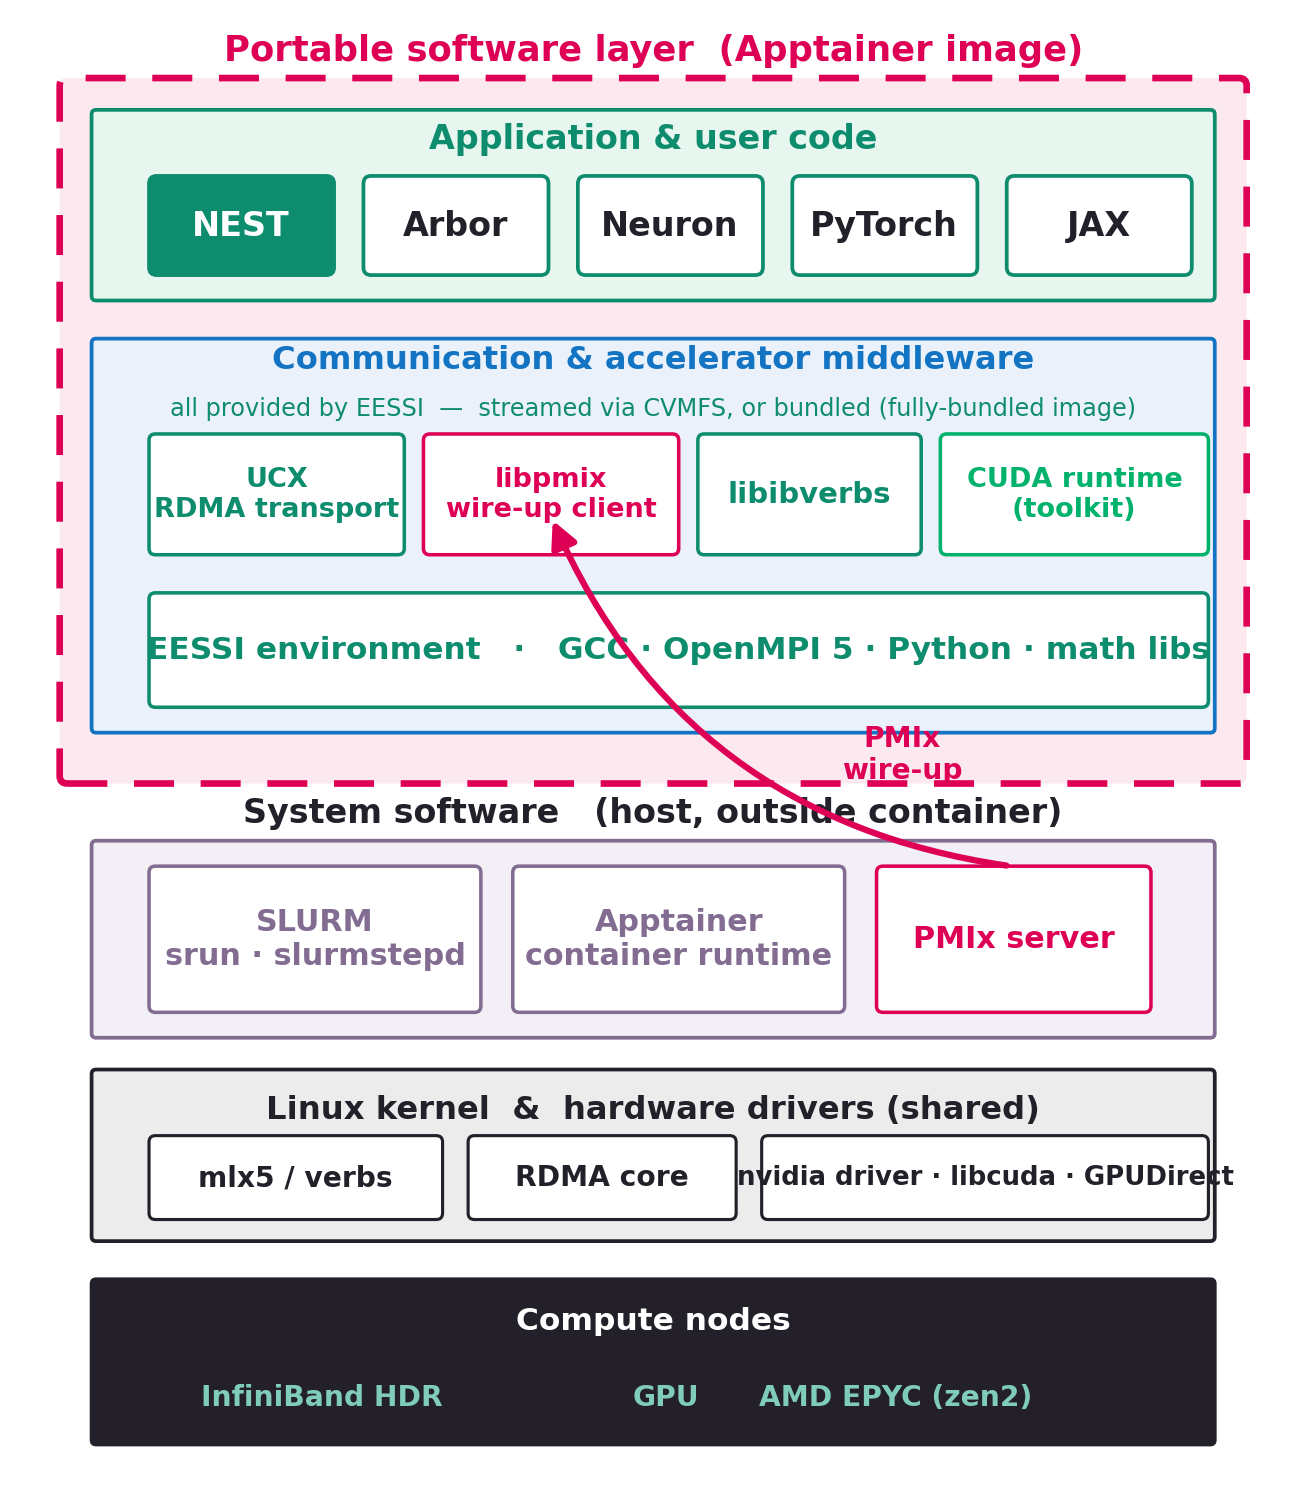
\includegraphics[width=0.86\textwidth]{figures/arch_layers.png}\\[-0.2cm]
        {\small Host\,/\,container split; magenta = PMIx wire-up.}
      \end{column}
      \begin{column}{0.52\textwidth}
        \centering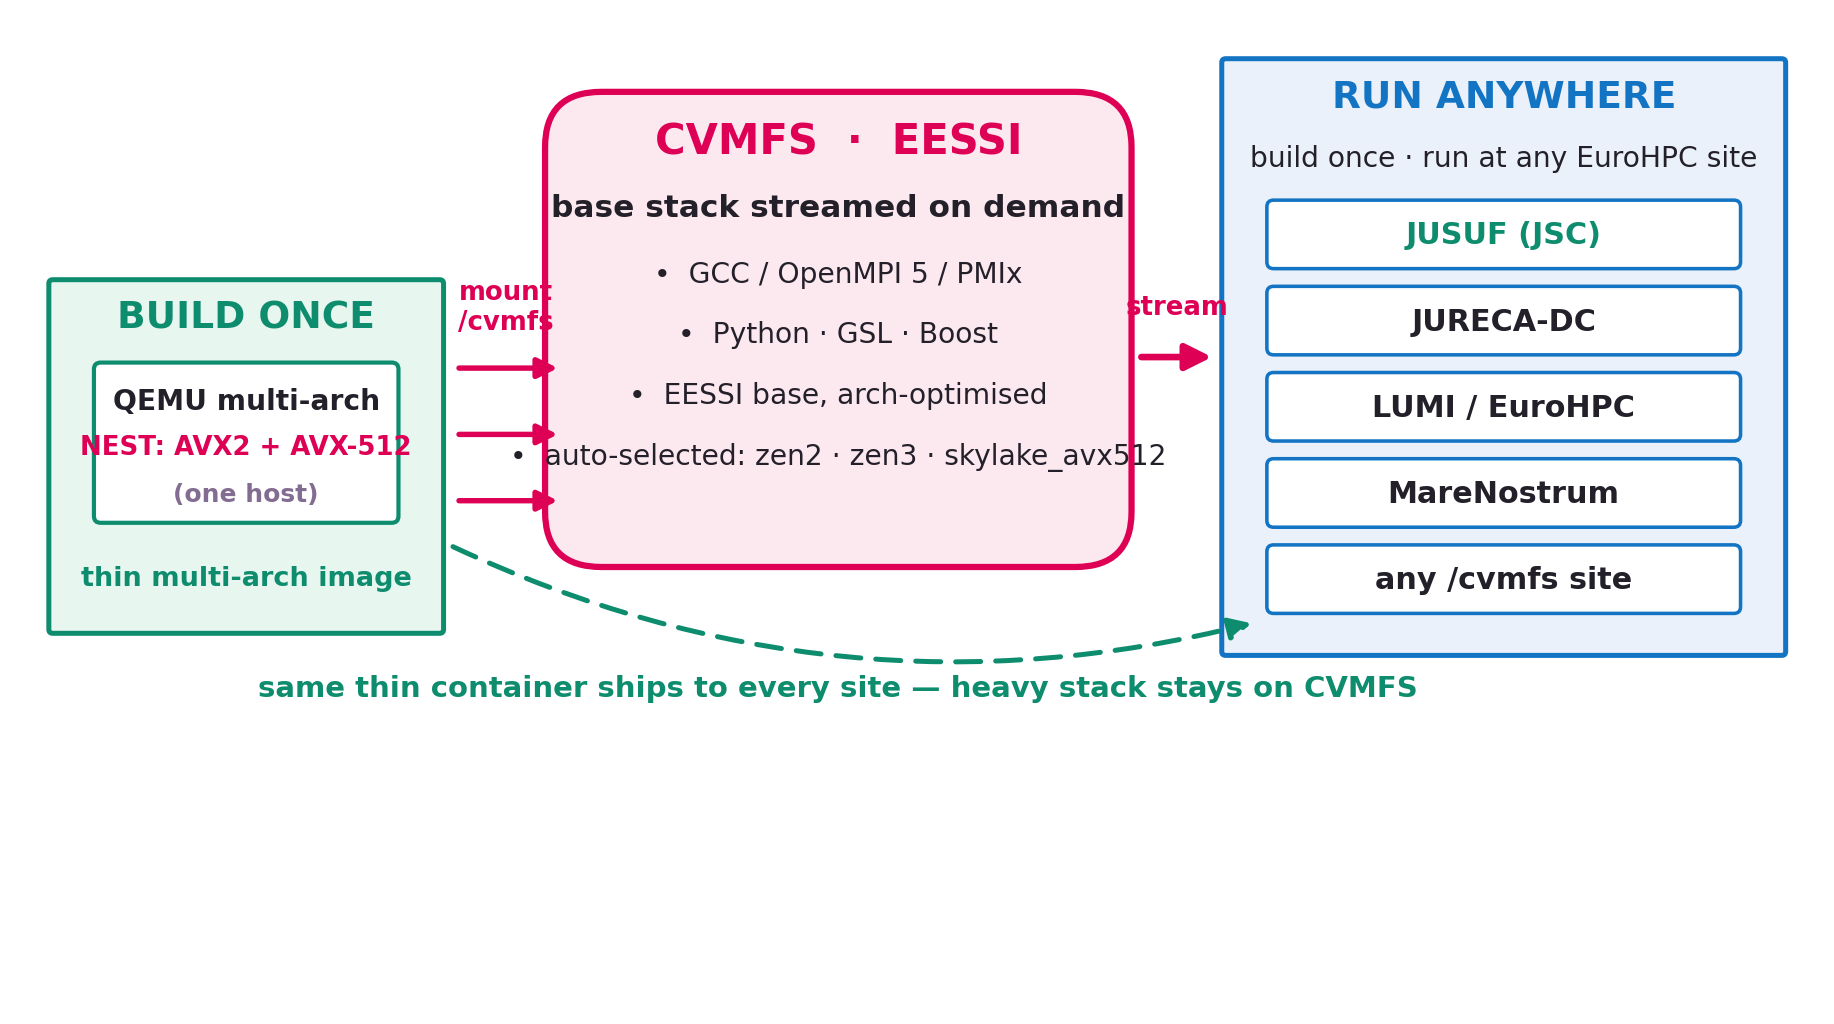
\includegraphics[width=0.98\textwidth]{figures/cvmfs_streaming.png}\\[0.2cm]
        {\small Build once $\rightarrow$ stream stack from CernVM-FS $\rightarrow$ run at any EuroHPC site.}
      \end{column}
    \end{columns}
    \vspace{0.3cm}

    % ---- table, full width beneath the figures ----
    \heading{Dependency provenance across deployment models}
    {\centering\normalsize
    \renewcommand{\arraystretch}{1.3}\setlength{\tabcolsep}{10pt}
    \begin{tabular}{@{}l c c c@{}}
      \textbf{Software component} & \tl{Bare-metal} & \textcolor{ebrmag}{\textbf{CVMFS-streamed}} & \textcolor{ebrviolet}{\textbf{Fully-bundled}}\\
      \hline
      OS userspace & \cH & \cI & \cI\\
      Application: \textbf{NEST} & \cM & \cI & \cI\\
      MPI \& comm.~(OpenMPI, UCX, PMIx) & \cM & \cC & \cI\\
      Base libraries (GCC, Python, math) & \cM & \cC & \cI\\
      PMIx server $\cdot$ fabric $\cdot$ drivers & \cH & \cH & \cH\\
    \end{tabular}\par}
  \end{column}
\end{columns}
\end{block}
